\documentclass[11pt,a4paper]{article}

\usepackage[margin=1in]{geometry}
\usepackage{amsmath,amssymb,mathtools}
\usepackage{booktabs,longtable,array}
\usepackage{enumitem}
\usepackage{xcolor}
\usepackage{hyperref}
\usepackage{fancyhdr}
\usepackage{titlesec}
\usepackage{microtype}
\usepackage[T1]{fontenc}
\usepackage{lmodern}
\usepackage{listings}
\usepackage{caption}
\usepackage{float}
\usepackage{tikz}
\usetikzlibrary{arrows.meta,positioning,shapes.geometric}

\definecolor{navy}{HTML}{0F172A}
\definecolor{cyanx}{HTML}{0891B2}
\definecolor{violetx}{HTML}{7C3AED}
\definecolor{softgray}{HTML}{64748B}
\definecolor{codebg}{HTML}{F8FAFC}

\hypersetup{
  colorlinks=true,
  linkcolor=violetx,
  urlcolor=cyanx,
  citecolor=violetx,
  pdftitle={QuantLab: Computational Finance and Scientific Machine Learning Workstation},
  pdfauthor={Rancy Chepchirchir}
}

\pagestyle{fancy}
\fancyhf{}
\lhead{QuantLab Technical Report}
\rhead{Rancy Chepchirchir}
\cfoot{\thepage}
\renewcommand{\headrulewidth}{0.3pt}

\titleformat{\section}{\Large\bfseries\color{navy}}{\thesection}{0.75em}{}
\titleformat{\subsection}{\large\bfseries\color{violetx}}{\thesubsection}{0.75em}{}

\lstset{
  backgroundcolor=\color{codebg},
  basicstyle=\ttfamily\small,
  frame=single,
  rulecolor=\color{softgray!25},
  breaklines=true,
  columns=fullflexible,
  showstringspaces=false
}

\title{\textbf{QuantLab}\\[0.4em]
\Large Computational Finance \& Scientific Machine Learning Workstation\\[0.8em]
\large A Step-by-Step Technical and Research Development Report}
\author{Rancy Chepchirchir}
\date{2 September 2026}

\begin{document}
\maketitle

\begin{abstract}
QuantLab is an interactive computational-finance research workstation developed to compare analytical pricing, lattice methods, finite-difference PDE solvers, Monte Carlo simulation, implied-volatility models, and physics-informed neural networks within a common experimental environment. The project began as an option-pricing comparison application and evolved into a broader research platform with four principal modules: Pricing Lab, Volatility Lab, Surface Atlas, and Research Lab. This report records the project chronologically, explains the mathematical methods, documents key implementation and deployment decisions, describes the American Option Surface Atlas and PINN convergence experiments in detail, and preserves the scientific cautions needed for future work. The report is intended both as project documentation and as a technical notebook that can support future thesis, paper, portfolio, and research-development work.
\end{abstract}

\tableofcontents
\newpage

\section{Project Vision}

QuantLab was built around a simple but increasingly important question: how should classical numerical finance and modern scientific machine learning be compared in a way that is computationally reproducible, visually interpretable, and scientifically honest?

Rather than building a collection of unrelated calculators, the project uses shared contract assumptions and common reference grids so that methods can be compared directly. Its current public identity is:

\begin{quote}
\textbf{QuantLab -- Computational Finance \& Scientific Machine Learning Workstation.} An interactive research platform for option pricing, volatility modelling and scientific machine learning, combining analytical methods, numerical PDE solvers, Monte Carlo simulation and physics-informed neural networks.
\end{quote}

The current application structure is:

\begin{center}
\begin{tabular}{ll}
\toprule
Module & Route \\
\midrule
Pricing Lab & \texttt{/} \\
Volatility Lab & \texttt{/volatility-lab} \\
Surface Atlas & \texttt{/surface-atlas} \\
Research Lab & \texttt{/research-lab} \\
\bottomrule
\end{tabular}
\end{center}

The old concept of a separate ``Overview'' page was removed because the root route already functioned as the Pricing Lab. This simplified the information architecture and made the research modules first-class components of the application.

\section{System Architecture}

\subsection{Frontend}

The frontend is built with Next.js, React, TypeScript and Tailwind CSS. Recharts is used for two-dimensional quantitative graphics, while Plotly is used for interactive three-dimensional surfaces.

The visual design evolved toward a dark scientific-workstation aesthetic: dense analytical grids, navy/purple/cyan accents, compact metric cards, and research-oriented surface plots rather than a conventional financial dashboard.

\subsection{Backend}

The backend is implemented in FastAPI and relies on NumPy and SciPy for numerical methods. Pydantic is used for typed API models. HTTPX/Requests support external data-provider abstractions where required.

\subsection{Deployment and CI}

The backend is deployed on Railway and the frontend on Vercel. GitHub Actions provides continuous integration. A key deployment constraint is that PyTorch is not part of the production backend requirements.

\subsection{Offline scientific-ML architecture}

PINNs are trained offline. The trained experiment outputs are exported as JSON artifacts and consumed by the production API using lightweight numerical interpolation. This prevents an API request from initiating expensive retraining and keeps production deployment independent of PyTorch.

The architecture can be summarized as follows:

\begin{figure}[H]
\centering
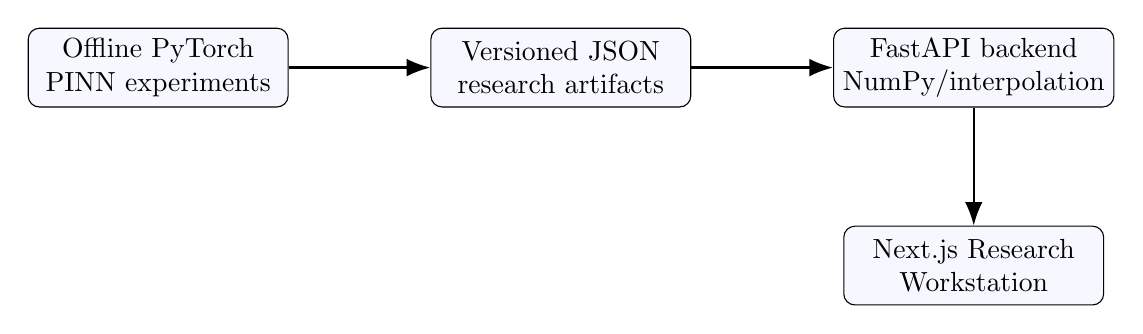
\begin{tikzpicture}[
  node distance=1.5cm and 1.8cm,
  box/.style={draw,rounded corners,align=center,minimum width=3.3cm,minimum height=1cm,fill=blue!3},
  arr/.style={-{Latex[length=3mm]},thick}
]
\node[box] (train) {Offline PyTorch\\PINN experiments};
\node[box,right=of train] (json) {Versioned JSON\\research artifacts};
\node[box,right=of json] (api) {FastAPI backend\\NumPy/interpolation};
\node[box,below=of api] (front) {Next.js Research\\Workstation};
\draw[arr] (train) -- (json);
\draw[arr] (json) -- (api);
\draw[arr] (api) -- (front);
\end{tikzpicture}
\caption{Production architecture for PINN research outputs. Training is deliberately separated from runtime serving.}
\end{figure}

\section{Version 1: Pricing Foundations}

\subsection{Shared pricing experiment}

The first version established a common pricing input model containing spot price, strike, risk-free rate, volatility, maturity, dividend yield and option type. Multiple pricing engines are evaluated under the same market assumptions.

The principal methods were:

\begin{itemize}[leftmargin=2em]
\item Black--Scholes analytical pricing;
\item Cox--Ross--Rubinstein binomial pricing;
\item Crank--Nicolson finite differences;
\item Monte Carlo simulation;
\item Black--Scholes Greeks;
\item spot sweeps and sensitivity plots;
\item numerical convergence experiments;
\item accuracy-versus-runtime comparisons.
\end{itemize}

\subsection{Black--Scholes benchmark}

For a European call with continuous dividend yield \(q\),

\[
C=S_0e^{-qT}N(d_1)-Ke^{-rT}N(d_2),
\]

where

\[
d_1=\frac{\ln(S_0/K)+(r-q+\tfrac12\sigma^2)T}{\sigma\sqrt{T}},
\qquad
 d_2=d_1-\sigma\sqrt{T}.
\]

Where an analytical solution exists, it provides a convenient benchmark for lattice, finite-difference and Monte Carlo convergence.

\subsection{CRR lattice}

The CRR tree approximates the underlying diffusion using

\[
u=e^{\sigma\sqrt{\Delta t}},\qquad d=u^{-1},
\]

with risk-neutral probability

\[
p=\frac{e^{(r-q)\Delta t}-d}{u-d}.
\]

For American options, backward induction applies the exercise projection

\[
V=\max\{V_{\text{continuation}},\Phi(S)\}
\]

at each node.

\subsection{Finite differences}

The Black--Scholes PDE is

\[
\frac{\partial V}{\partial t}
+(r-q)S\frac{\partial V}{\partial S}
+\frac12\sigma^2S^2\frac{\partial^2V}{\partial S^2}
-rV=0.
\]

Crank--Nicolson averages the explicit and implicit time discretizations. During early development, the comparison endpoint was improved by using an efficient tridiagonal solution structure instead of a computationally expensive dense approach.

\subsection{Monte Carlo}

Risk-neutral terminal prices are sampled from

\[
S_T=S_0\exp\left[
\left(r-q-\frac12\sigma^2\right)T+
\sigma\sqrt{T}Z
\right],
\qquad Z\sim N(0,1).
\]

The discounted payoff estimator is

\[
\hat V=e^{-rT}\frac{1}{M}\sum_{m=1}^{M}\Phi(S_T^{(m)}).
\]

The Pricing Lab reports both approximation error and Monte Carlo uncertainty, making stochastic sampling visibly different from deterministic discretization error.

\subsection{Convergence Lab}

The frontend includes convergence plots for lattice refinement and Monte Carlo sampling. This was an early step toward the central QuantLab idea: methods should be compared through convergence and computational cost, not only through final prices.

\section{Version 2: Implied Volatility and Surface Modelling}

V2 extended QuantLab from option-value computation to market-implied volatility structure.

\subsection{Implied-volatility inversion}

Given a market price \(P_{\mathrm{mkt}}\), implied volatility solves

\[
P_{\mathrm{model}}(\sigma_{\mathrm{impl}})-P_{\mathrm{mkt}}=0.
\]

A robust bisection procedure was implemented. For American options, CRR pricing can be used inside the inversion loop when exercise optionality invalidates a direct European Black--Scholes inversion.

\subsection{Surface modelling}

The volatility module grew to include interpolation, raw SVI and SSVI representations, model comparisons, calibration and arbitrage diagnostics.

A generic SVI slice can be written as

\[
w(k)=a+b\left\{\rho(k-m)+\sqrt{(k-m)^2+\sigma^2}\right\},
\]

where \(k\) is log-moneyness and \(w\) total implied variance.

\subsection{Scientific cautions}

Several correctness decisions were made during this phase:

\begin{itemize}[leftmargin=2em]
\item butterfly tests must not average call and put prices;
\item the option type used in market butterfly diagnostics must be internally consistent;
\item SVI/SSVI surfaces in the implemented workflow are European-call constructions;
\item fixed-strike total-variance calendar checks are diagnostics rather than universal proofs of static-arbitrage freedom.
\end{itemize}

These distinctions should remain visible in future documentation and UI labels.

\section{Version 3: Research Workstation}

The third phase changed QuantLab from a conventional quantitative-finance application into a more explicit research environment.

Major additions included a shared shell, research navigation, dense KPI strips, compact market controls, 3D volatility surfaces, SSVI total-variance visualization and, most importantly, the American Option Surface Atlas.

\section{American Option Surface Atlas}

\subsection{Why American puts?}

The current projected Crank--Nicolson implementation is designed for American puts. This makes the put the natural instrument for studying the obstacle problem, the stopping region and the numerical free boundary.

\subsection{Variational inequality}

For payoff \(\Phi(S)\), the American pricing problem is

\[
\max\left\{
\frac{\partial V}{\partial t}
+(r-q)S V_S
+\frac12\sigma^2S^2V_{SS}
-rV,
\Phi(S)-V
\right\}=0,
\qquad V(T,S)=\Phi(S).
\]

For a put,

\[
\Phi(S)=\max(K-S,0).
\]

The Surface Atlas uses time-to-maturity

\[
\tau=T-t,
\]

so plots run naturally from maturity backward into longer time remaining.

\subsection{Projected Crank--Nicolson}

A numerical CN candidate is projected onto the obstacle:

\[
V_i^n=\max\left(V_i^{n,\mathrm{CN}},\Phi(S_i)\right).
\]

This produces a practical numerical reference surface. It must not be called an exact solution.

\subsection{Common comparison grid}

CRR produces scalar prices at requested state points while CN naturally produces a rectangular space-time grid. To compare the two methods, CRR values are evaluated on the same common grid used for the research atlas.

The signed error surface is

\[
E_{\mathrm{CRR}}(S,\tau)=V_{\mathrm{CRR}}(S,\tau)-V_{\mathrm{CN}}(S,\tau).
\]

\subsection{Exercise gap and free-boundary estimate}

Define

\[
G(S,\tau)=V(S,\tau)-\max(K-S,0).
\]

This is an exercise/continuation gap, not a discretization error.

A numerical boundary estimate can be written

\[
S^*(\tau)\approx\sup\{S_i<K:G(S_i,\tau)\le\epsilon\}.
\]

The resulting boundary is a diagnostic extracted from the discretized reference surface.

\subsection{Poster-style analytical matrix}

The atlas design intentionally uses small multiples because they support method-to-method comparison better than a single oversized 3D plot. The early matrix included CRR, CN, signed error, exercise gap and free-boundary visualizations. This structure later became the basis for PINN comparison panels.

\section{Physics-Informed Neural Network Experiment}

\subsection{Model formulation}

The PINN approximates the option value \(V_\theta(S,t)\) with a Tanh network. Rather than treating the American obstacle as an ordinary equality PDE, the experiment incorporates complementarity through a smoothed Fischer--Burmeister function

\[
\phi_\epsilon(a,b)
=\sqrt{a^2+b^2+\epsilon^2}-a-b,
\]

where

\[
a=V-\Phi,
\qquad
b=-\mathcal{L}V.
\]

Here \(\mathcal{L}\) denotes the Black--Scholes differential operator including discounting.

\subsection{Training configuration}

The existing V2 experiment uses a representative configuration of 4000 epochs, 3000 interior points, 1000 terminal samples, 1000 boundary samples, learning rate \(10^{-3}\), complementarity weight 10, terminal/boundary weights 5 and seed 42.

The base contract family in the stored experiment is

\[
K=100,\quad r=0.05,\quad \sigma=0.20,\quad T=1,\quad q=0.
\]

\subsection{Coordinate conversion}

The PINN was trained in calendar time \(t\), whereas Surface Atlas visualizes \(\tau=T-t\). This transformation is required before interpolation and comparison. Forgetting it would silently misalign surfaces while still producing visually plausible plots.

\subsection{Offline artifacts}

Two important stored artifacts are:

\begin{lstlisting}
backend/experiments/results/american_pinn_v2_surface.json
backend/experiments/results/american_pinn_convergence_atlas.json
\end{lstlisting}

The convergence experiment captures snapshots at 500, 1000, 2000 and 4000 epochs from a single training trajectory.

\section{PINN Error Topography and Learning Dynamics}

\subsection{Reference error}

PINN error is measured against projected CN:

\[
E_{\mathrm{PINN}}(S,\tau)
=V_{\mathrm{PINN}}(S,\tau)-V_{\mathrm{CN}}(S,\tau).
\]

Absolute error is

\[
|E_{\mathrm{PINN}}(S,\tau)|.
\]

The language ``exact error'' is intentionally avoided because CN is a numerical reference.

\subsection{Improvement surface}

To visualize where training made progress,

\[
I_{500\to4000}(S,\tau)
=|E_{500}(S,\tau)|-|E_{4000}(S,\tau)|.
\]

Positive regions indicate a reduction in absolute error between early and late training.

\subsection{Boundary-distance profile}

A grid-aware distance is used:

\[
\Delta S=\operatorname{median}(S_{i+1}-S_i),
\qquad
 d_h=\frac{|S-S^*(\tau)|}{\Delta S}.
\]

The error field is summarized in bands such as \(<1\Delta S\), \(1-2\Delta S\), \(2-4\Delta S\), \(4-8\Delta S\), and \(8+\Delta S\).

The observed training trajectory supports a descriptive picture of broad-domain error gradually collapsing into more localized residual structure. This is informative evidence but should not be overstated as a formal causal result.

\section{Linear and Logarithmic Error Views}

The PINN Error-Evolution Atlas now supports two complementary display modes.

\subsection{Linear scale}

\[
z=|E|.
\]

A pooled 97.5th-percentile upper display limit is used across all four checkpoints. This prevents a few large early errors from visually flattening the converged surface while preserving the true uncapped maximum as a reported metric.

\subsection{Logarithmic scale}

\[
z=\log_{10}(\max(|E|,10^{-6})).
\]

The log view exposes low-magnitude residual geometry that cannot be read easily on a linear scale. Importantly, MAE, RMSE and maximum-error cards remain in the original price-error units. Only the display coordinate is transformed.

The free-boundary ridge must be transformed consistently into the same z coordinate in log mode.

\section{Frontend WebGL Failure and Resolution}

\subsection{Observed failure}

After several new 3D PINN panels were mounted simultaneously, the top CRR panel became a large white region. Browser logs reported a Plotly/WebGL shader compilation failure.

Because the same generic surface component worked for CN and PINN, the initial possibility of corrupt CRR data was tested directly by removing the lower multi-surface error-evolution component. The CRR surface immediately rendered again.

\subsection{Diagnosis}

The failure was caused by browser WebGL context/resource pressure rather than pricing data or Plotly trace configuration.

\subsection{Architectural fix}

A reusable lazy section was introduced using \texttt{IntersectionObserver}. Lower 3D components mount when approaching the viewport and may unmount when hidden. This releases WebGL contexts and allows the primary method atlas to stay eager.

This fix is more robust than modifying arbitrary plot parameters because it addresses the actual resource lifecycle.

\section{Navigation and Portfolio Integration}

The V3 sidebar was simplified so that the main route is explicitly Pricing Lab. Surface Atlas was added as a first-class navigation destination and promoted through a CTA on the main page.

The portfolio-ready information architecture is therefore:

\begin{lstlisting}
Pricing Lab       /
Volatility Lab    /volatility-lab
Surface Atlas     /surface-atlas
Research Lab      /research-lab
\end{lstlisting}

A concise portfolio description is:

\begin{quote}
\textbf{QuantLab -- Computational Finance \& Scientific Machine Learning Workstation.} An interactive research platform for option pricing, volatility modelling and scientific machine learning, combining analytical methods, numerical PDE solvers, Monte Carlo simulation and physics-informed neural networks.
\end{quote}

The recommended project status is ``Active research project'' rather than ``finished'', because the existing application already tells a coherent technical story while leaving room for further research.

\section{Testing, CI and Repository Discipline}

Backend tests were run through Pytest with the backend package on \texttt{PYTHONPATH}. Tests associated with the new Surface Atlas initially exposed stale assumptions about grid dimensions and an obsolete surface-field name. These were corrected to reflect the actual common comparison grid and current dataclass/API fields.

Generated experiment PNGs are intentionally ignored, while compact JSON artifacts needed by the runtime architecture are versioned. This separates reproducible research data from disposable render outputs.

A meaningful repository checkpoint was committed under the message:

\begin{quote}
\texttt{feat: add American option surface atlas and PINN boundary diagnostics}
\end{quote}

and later frontend integration was committed as:

\begin{quote}
\texttt{feat: integrate Surface Atlas into QuantLab workstation}
\end{quote}

\section{Scientific Interpretation: What QuantLab Can and Cannot Claim}

The project now supports several strong statements:

\begin{itemize}[leftmargin=2em]
\item numerical and learned American-option surfaces can be compared on a common state-time grid;
\item PINN approximation error can be studied spatially rather than reduced to a single scalar metric;
\item the training trajectory can be inspected at multiple checkpoints;
\item residual error becomes substantially smaller and more spatially localized across the stored trajectory;
\item meaningful residual structure appears near the numerically estimated stopping boundary in the converged regime.
\end{itemize}

However, the following claims should be avoided without additional experiments:

\begin{itemize}[leftmargin=2em]
\item projected CN is an exact American-option solution;
\item all residual error near the stopping region is caused by free-boundary learning difficulty;
\item a single Pearson distance-error correlation proves boundary concentration;
\item the current one-parameter PINN generalizes as an operator across contract families;
\item the current results establish superiority of PINNs over numerical methods.
\end{itemize}

\section{Future Research Roadmap}

\subsection{Near-term: improve the existing experiment}

The most natural future steps are not additional dashboard features but improvements in research validity:

\begin{enumerate}[leftmargin=2em]
\item Promote the strongest converged PINN checkpoint for default comparison while preserving early checkpoints for learning-dynamics analysis.
\item Increase projected-CN resolution and conduct grid-refinement studies.
\item Quantify sensitivity of the extracted free boundary to grid spacing and gap threshold.
\item Separate terminal/spatial-boundary residuals from stopping-boundary residuals if a publication-level attribution is required.
\end{enumerate}

\subsection{Numerical-method extensions}

Potential baselines include trinomial lattices, explicit/implicit finite differences, adaptive meshes, Richardson extrapolation and Longstaff--Schwartz Monte Carlo.

The purpose should remain a structured comparison of approximation behaviour rather than a feature checklist.

\subsection{Scientific-ML extensions}

A major research direction is a parameter-conditioned approximation

\[
V_\theta(S,K,r,q,\sigma,\tau),
\]

which moves the problem toward learning an option-pricing operator instead of fitting a single PDE instance. DeepONet or related operator-learning architectures become more meaningful in that setting.

Uncertainty-aware extensions could include ensembles, Bayesian approximations, conformal calibration or explicit uncertainty over learned-model discrepancy.

\subsection{Volatility extensions}

Possible future work includes SABR, Heston calibration, local volatility, temporal SVI/SSVI stability, calibration uncertainty and more systematic surface-arbitrage stress tests.

\subsection{Surface Atlas as flagship interface}

Potential research-interface improvements include maturity slices, method-to-method boundary comparisons, parameter-sweep atlases, training animations, click-to-expand small multiples and an export-ready figure mode for papers and presentations.

Because Plotly 3D surfaces consume WebGL contexts, future visual expansion should preserve lazy mounting rather than rendering every possible surface simultaneously.

\section{Recommended Documentation Structure}

QuantLab should maintain three complementary documentation layers:

\begin{enumerate}[leftmargin=2em]
\item a concise repository \texttt{README.md};
\item a living research journal recording dated decisions and future ideas;
\item this formal LaTeX/PDF report, which can grow into thesis or paper documentation.
\end{enumerate}

A useful habit is to add a dated journal entry after each major experiment, especially when a scientific interpretation or architecture decision changes.

\section{Current Checkpoint: 2 September 2026}

At this checkpoint:

\begin{itemize}[leftmargin=2em]
\item QuantLab is portfolio-ready.
\item The root page is the canonical Pricing Lab.
\item Surface Atlas is a first-class module and is linked from the main page.
\item American put surfaces compare CRR, projected CN and PINN outputs.
\item PINN convergence checkpoints at 500, 1000, 2000 and 4000 epochs are available.
\item Linear and log error-evolution views are implemented.
\item The free-boundary ridge is displayed consistently in both scales.
\item the WebGL multi-surface failure has been fixed using lazy plot mounting.
\item frontend integration changes have been committed and pushed.
\end{itemize}

The next practical task is portfolio integration: use a strong Surface Atlas image as the visual anchor, provide Live Demo and GitHub links, summarize the four research modules, and present QuantLab as active computational-finance research software.

\section{Closing Note to Future Me}

QuantLab became interesting when it stopped being merely an option-pricing interface and started asking where approximations fail, how error changes during training, and what the geometry of numerical and learned solutions reveals. Preserve that direction.

When considering a new feature, ask three questions:

\begin{enumerate}[leftmargin=2em]
\item What research question does this answer?
\item What is the comparison or benchmark that makes the result meaningful?
\item Can the visualization distinguish a scientific phenomenon from an implementation artifact?
\end{enumerate}

If those questions do not yet have good answers, the feature can wait.

\end{document}
